\documentclass[]{article}\usepackage[]{graphicx}\usepackage[]{color}
%% maxwidth is the original width if it is less than linewidth
%% otherwise use linewidth (to make sure the graphics do not exceed the margin)
\makeatletter
\def\maxwidth{ %
  \ifdim\Gin@nat@width>\linewidth
    \linewidth
  \else
    \Gin@nat@width
  \fi
}
\makeatother

\definecolor{fgcolor}{rgb}{0.345, 0.345, 0.345}
\newcommand{\hlnum}[1]{\textcolor[rgb]{0.686,0.059,0.569}{#1}}%
\newcommand{\hlstr}[1]{\textcolor[rgb]{0.192,0.494,0.8}{#1}}%
\newcommand{\hlcom}[1]{\textcolor[rgb]{0.678,0.584,0.686}{\textit{#1}}}%
\newcommand{\hlopt}[1]{\textcolor[rgb]{0,0,0}{#1}}%
\newcommand{\hlstd}[1]{\textcolor[rgb]{0.345,0.345,0.345}{#1}}%
\newcommand{\hlkwa}[1]{\textcolor[rgb]{0.161,0.373,0.58}{\textbf{#1}}}%
\newcommand{\hlkwb}[1]{\textcolor[rgb]{0.69,0.353,0.396}{#1}}%
\newcommand{\hlkwc}[1]{\textcolor[rgb]{0.333,0.667,0.333}{#1}}%
\newcommand{\hlkwd}[1]{\textcolor[rgb]{0.737,0.353,0.396}{\textbf{#1}}}%
\let\hlipl\hlkwb

\usepackage{framed}
\makeatletter
\newenvironment{kframe}{%
 \def\at@end@of@kframe{}%
 \ifinner\ifhmode%
  \def\at@end@of@kframe{\end{minipage}}%
  \begin{minipage}{\columnwidth}%
 \fi\fi%
 \def\FrameCommand##1{\hskip\@totalleftmargin \hskip-\fboxsep
 \colorbox{shadecolor}{##1}\hskip-\fboxsep
     % There is no \\@totalrightmargin, so:
     \hskip-\linewidth \hskip-\@totalleftmargin \hskip\columnwidth}%
 \MakeFramed {\advance\hsize-\width
   \@totalleftmargin\z@ \linewidth\hsize
   \@setminipage}}%
 {\par\unskip\endMakeFramed%
 \at@end@of@kframe}
\makeatother

\definecolor{shadecolor}{rgb}{.97, .97, .97}
\definecolor{messagecolor}{rgb}{0, 0, 0}
\definecolor{warningcolor}{rgb}{1, 0, 1}
\definecolor{errorcolor}{rgb}{1, 0, 0}
\newenvironment{knitrout}{}{} % an empty environment to be redefined in TeX

\usepackage{alltt}
%\usepackage[landscape, margin=0.1in]{geometry}
%\usepackage[margin=0.1in]{geometry}
\usepackage[left=0.1in, bottom=0.1in, top=0.1in, right=0.3in]{geometry}
\usepackage{grid-system}
\renewcommand{\familydefault}{\sfdefault}
\usepackage{setspace}			% \doublespacing
\usepackage{graphicx}
\usepackage{graphbox} 		% loads graphicx package			Not sure if I'm using this
\usepackage{xcolor}				% textbox colors (I think being used by \fcolorbox)
\usepackage{hyperref}
\hypersetup{
	colorlinks=true,
	linkcolor=cyan,
	filecolor=magenta, 
	urlcolor=blue
}

\usepackage{fancyhdr}
\usepackage{lastpage}		% For \pageref{LastPage}
\pagestyle{fancy}
\fancyhf{}
% Manually adjust the vertical space in the header and footer to account for narrow 
%   margins. This is kludgy.
%\rhead{\vspace{1.2cm} {\footnotesize \emph{Report Version 1.1, Updated 2019-02-15}}}
\rfoot{\vspace{-1.5cm} Page \thepage \hspace{1pt} of \pageref*{LastPage}}
\renewcommand{\headrulewidth}{0pt}		% Get rid of fancyhdr's vertical lines
\renewcommand{\footrulewidth}{0pt}		% Get rid of fancyhdr's vertical lines

\usepackage{parskip}		% Bullets close together

% Using this instead of base itemize because it allows for easier customization of 
%   margins:
\usepackage{enumitem}			% [leftmargin=*]
%\renewcommand\labelitemi{\tiny$\bullet$}		% smaller itemize bullets

\setlength{\fboxsep}{5pt}		% fcolorbox margins
%%%%%%%%%%%%%%%%%%%%%%%%%%%%%%%%%%%%%%%%%%%%%%%%%%%%%%%%%%%%%%
\IfFileExists{upquote.sty}{\usepackage{upquote}}{}
\begin{document}




%%%% Secchi Depth:
\begin{Row}
  \begin{Cell}{7}
    \vspace{0.2cm}
    \begin{center}
      \doublespacing
      {\Large Interagency Ecological Program Status \& Trends } \\
      \vspace{0.2cm}
      {\Large 2017-2018 Winter Season Report} \\
      \vspace{0.5cm}
      {\Huge Secchi Depth} \\
      \vspace{0.75cm}
      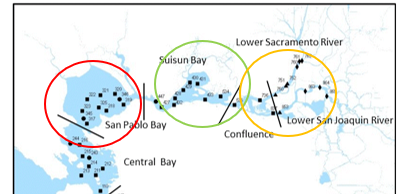
\includegraphics[width=8cm,align=m]{figures/region_map.png}
    \end{center}
  \end{Cell}
  \begin{Cell}{6}
    \vspace{0.2cm}
    \begin{center}
      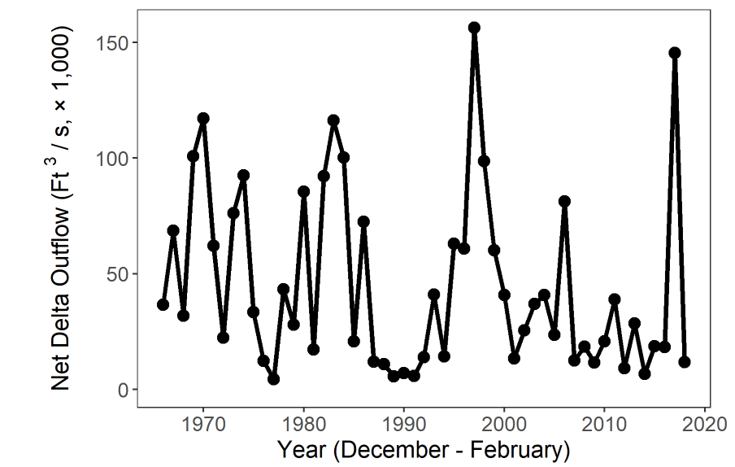
\includegraphics[width=7cm,trim=0 0 0 0,clip,align=m]{figures/outflow_tmp.png}
      \begin{itemize}[leftmargin=*]
        \item Delta outflow is a major ecosystem driver and depends on natural 
        hydrological variability and water management operations, including exports 
        from the Delta and reservoir operations. 
      \end{itemize}
    \end{center}
  \end{Cell}
\end{Row}

\vspace{1cm}

\begin{Row}
  \begin{Cell}{7}
    \begin{center}
      %\begin{minipage}{9cm}
        \begin{itemize}[leftmargin=1cm,rightmargin=1cm]
          \item Organisms in this ecosystem are adapted to high turbidity conditions, 
          and reductions in turbidity can have many negative ecological effects. Higher 
          values for Secchi depth indicate lower turbidity.
          \item Secchi depth is measured monthly by DWR’s Environmental monitoring 
          program by dropping a black-and-white disk in the water until it disappears.
        \end{itemize}
        \vspace{0.5cm}
        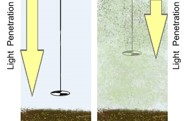
\includegraphics[width=6cm,align=m]{figures/secchi/secchi_diagram.jpg}
      %\end{minipage}
    \end{center}
  \end{Cell}
  \begin{Cell}{6}
    \begin{center}
      {\bf {\large Suisun Bay}}
      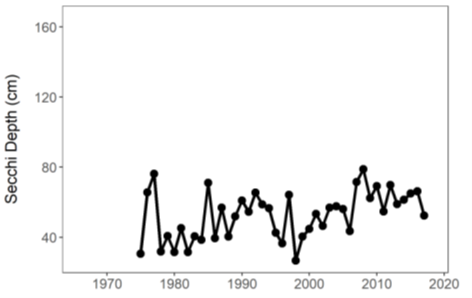
\includegraphics[width=9.5cm,align=m]{figures/secchi/secchi_suisun_bay_tmp.png}
      \vspace{0.5cm}
      \begin{itemize}[leftmargin=2cm,rightmargin=0.5cm]
        \item Suisun bay is usually pretty murkey, meaning low secchi depth.
      \end{itemize}
    \end{center}
  \end{Cell}
\end{Row}

\vspace{1cm}

\begin{Row}
  \begin{Cell}{7}
    \begin{center}
      {\bf {\large The Delta}}
      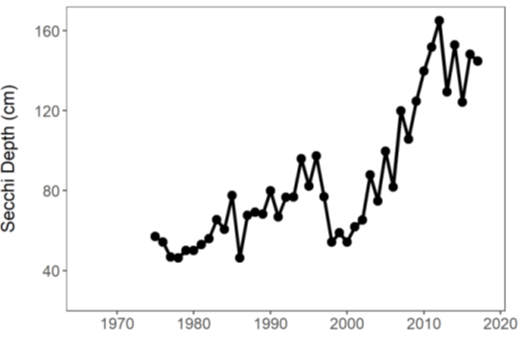
\includegraphics[width=9.5cm,align=m]{figures/secchi/secchi_delta_tmp.png}
      \vspace{0.5cm}
      \begin{itemize}[leftmargin=2cm,rightmargin=0.5cm]
        \item The Delta has been getting clearer over time.
      \end{itemize}
    \end{center}
  \end{Cell}
  \begin{Cell}{6}
    \begin{center}
      {\bf {\large San Pablo Bay}}
      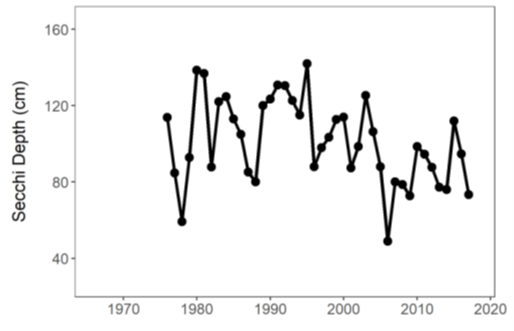
\includegraphics[width=9.5cm,align=m]{figures/secchi/secchi_san_pablo_bay_tmp.png}
      \vspace{0.5cm}
      \begin{itemize}[leftmargin=2cm,rightmargin=0.5cm]
        \item San Pablo bay is pretty clear.
      \end{itemize}
    \end{center}
  \end{Cell}
\end{Row}


\newpage


%%%% Temperature:
\begin{Row}
  \begin{Cell}{7}
    \vspace{0.2cm}
    \begin{center}
      \doublespacing
      {\Large Interagency Ecological Program Status \& Trends } \\
      \vspace{0.2cm}
      {\Large 2017-2018 Winter Season Report} \\
      \vspace{0.5cm}
      {\Huge Temperature} \\
      \vspace{0.75cm}
      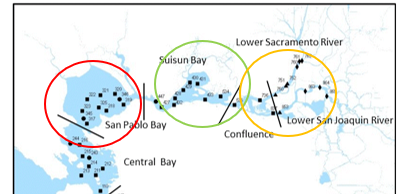
\includegraphics[width=8cm,align=m]{figures/region_map.png}
    \end{center}
  \end{Cell}
  \begin{Cell}{6}
    \vspace{0.2cm}
    \begin{center}
      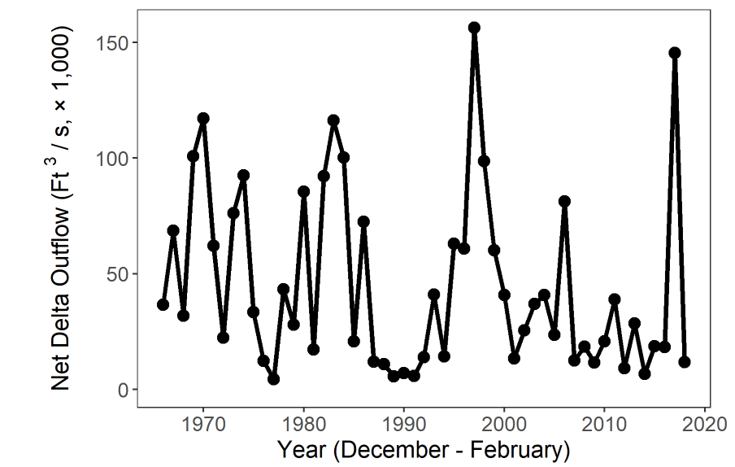
\includegraphics[width=7cm,trim=0 0 0 0,clip,align=m]{figures/outflow_tmp.png}
      \begin{itemize}[leftmargin=*]
        \item Delta outflow is a major ecosystem driver and depends on natural 
        hydrological variability and water management operations, including exports 
        from the Delta and reservoir operations. 
        \item High Delta outflow causes fresher conditions in San Pablo Bay.      
      \end{itemize}
    \end{center}
  \end{Cell}
\end{Row}

\vspace{1cm}

\begin{Row}
  \begin{Cell}{7}
    \begin{center}
      \begin{itemize}[leftmargin=1cm,rightmargin=1cm]
        \item Water temperature affects fish and stuff.
        \item High temperatures lead to fish not doing so good and some harmful 
        algal blooms.
        \item Climate change will make things worse.      
      \end{itemize}
      \vspace{0.5cm}
      
\includegraphics[width=4cm,align=m]{figures/temperature/temperature_graphic.png}
    \end{center}
  \end{Cell}
  \begin{Cell}{6}
    \begin{center}
      {\bf {\large Suisun Bay}}
      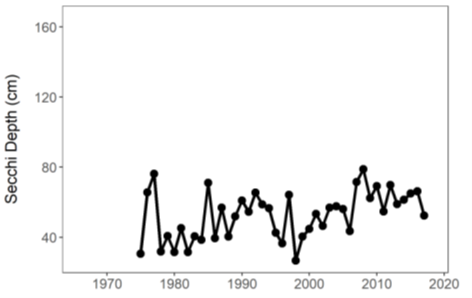
\includegraphics[width=9.5cm,align=m]{figures/temperature/temp_suisun_bay_tmp.png}
      \vspace{0.5cm}
      \begin{itemize}[leftmargin=2cm,rightmargin=0.5cm]
        \item Suisun Bay is cool.
      \end{itemize}
    \end{center}
  \end{Cell}
\end{Row}

\vspace{1cm}

\begin{Row}
  \begin{Cell}{7}
    \begin{center}
      {\bf {\large The Delta}}
      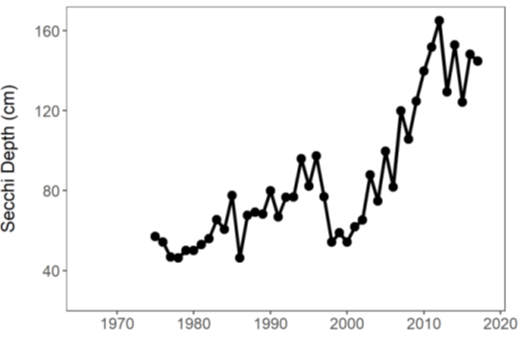
\includegraphics[width=9.5cm,align=m]{figures/temperature/temp_delta_tmp.png}
      \vspace{0.5cm}
      \begin{itemize}[leftmargin=2cm,rightmargin=0.5cm]
        \item The delta is hot and stuff, but wetlands might form thermal refugia.
      \end{itemize}
    \end{center}
  \end{Cell}
  \begin{Cell}{6}
    \begin{center}
      {\bf {\large San Pablo Bay}}
      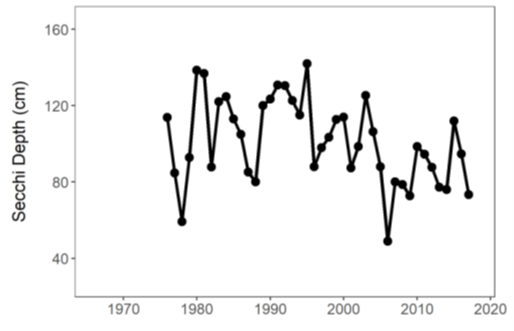
\includegraphics[width=9.5cm,align=m]{figures/temperature/temp_san_pablo_bay_tmp.png}
      \vspace{0.5cm}
      \begin{itemize}[leftmargin=2cm,rightmargin=0.5cm]
        \item Other fun temperature facts.
      \end{itemize}
    \end{center}
  \end{Cell}
\end{Row}


\newpage


%%%% Chlorophyll:
\begin{Row}
  \begin{Cell}{7}
    \vspace{0.2cm}
    \begin{center}
      \doublespacing
      {\Large Interagency Ecological Program Status \& Trends } \\
      \vspace{0.2cm}
      {\Large 2017-2018 Winter Season Report} \\
      \vspace{0.5cm}
      {\Huge Chlorophyll} \\
      \vspace{0.75cm}
      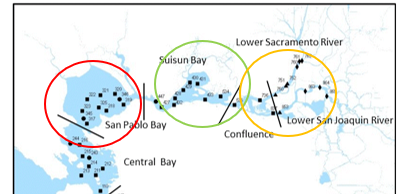
\includegraphics[width=8cm,align=m]{figures/region_map.png}
    \end{center}
  \end{Cell}
  \begin{Cell}{6}
    \vspace{0.2cm}
    \begin{center}
      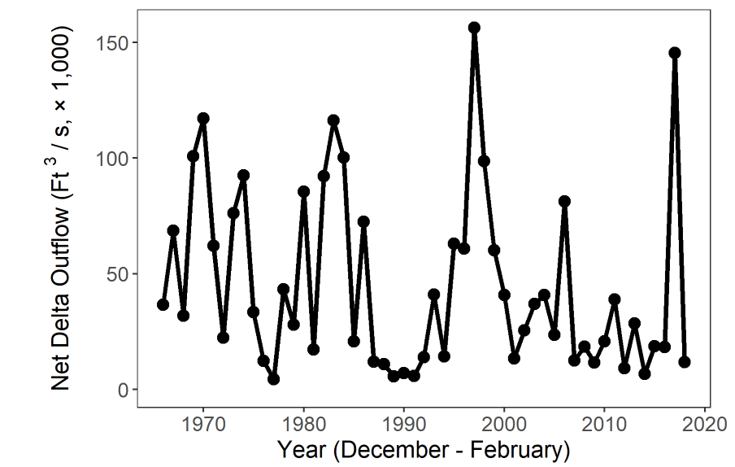
\includegraphics[width=7cm,trim=0 0 0 0,clip,align=m]{figures/outflow_tmp.png}
      \begin{itemize}[leftmargin=*]
        \item Delta outflow is a major ecosystem driver and depends on natural 
        hydrological variability and water management operations, including exports 
        from the Delta and reservoir operations. 
      \end{itemize}
    \end{center}
  \end{Cell}
\end{Row}

\vspace{1cm}

\begin{Row}
  \begin{Cell}{7}
    \begin{center}
      \begin{itemize}[leftmargin=1cm,rightmargin=1cm]
        \item Chlorophyll fact 1.
        \item Chlorophyll fact 2.
        \item Chlorophyll fact 3.
      \end{itemize}
      \vspace{0.5cm}
      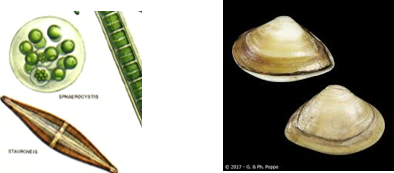
\includegraphics[width=8cm,align=m]{figures/chlorophyll/chlorophyll_pics.png}
    \end{center}
  \end{Cell}
  \begin{Cell}{6}
    \begin{center}
      {\bf {\large Suisun Bay}}
      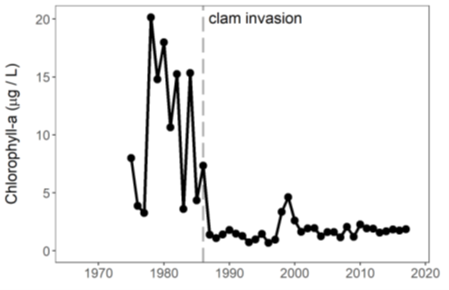
\includegraphics[width=9.5cm,align=m]{figures/chlorophyll/chlorophyll_suisun_bay_tmp.png}
      \vspace{0.5cm}
      \begin{itemize}[leftmargin=2cm,rightmargin=0.5cm]
        \item Clams really hit Suisun hard.
      \end{itemize}
    \end{center}
  \end{Cell}
\end{Row}

\vspace{1cm}

\begin{Row}
  \begin{Cell}{7}
    \begin{center}
      {\bf {\large The Delta}}
      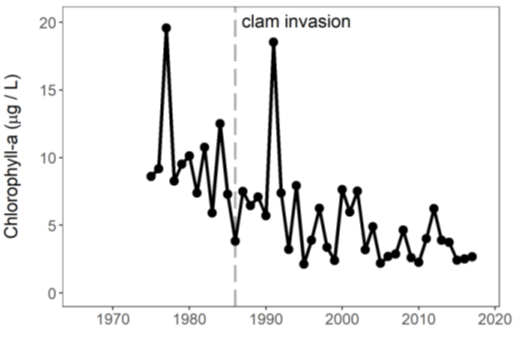
\includegraphics[width=9.5cm,align=m]{figures/chlorophyll/chlorophyll_delta_tmp.png}
      \vspace{0.5cm}
      \begin{itemize}[leftmargin=2cm,rightmargin=0.5cm]
        \item The delta is hot and stuff, but wetlands might form thermal refugia.
      \end{itemize}
    \end{center}
  \end{Cell}
  \begin{Cell}{6}
    \begin{center}
      {\bf {\large San Pablo Bay}}
      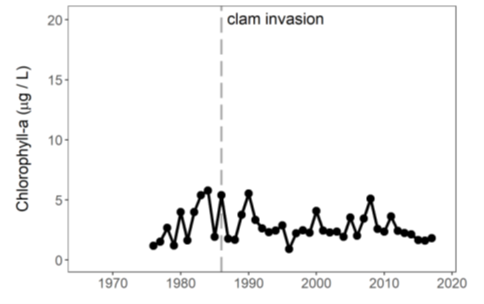
\includegraphics[width=9.5cm,align=m]{figures/chlorophyll/chlorophyll_san_pablo_bay_tmp.png}
      \vspace{0.5cm}
      \begin{itemize}[leftmargin=2cm,rightmargin=0.5cm]
        \item San Pablo bay didn't have a big decrease in chlorophyll after the clam 
        invasion, but it's always been low.
      \end{itemize}
    \end{center}
  \end{Cell}
\end{Row}


\newpage


%%%% Zooplankton:
\begin{Row}
  \begin{Cell}{7}
    \vspace{0.2cm}
    \begin{center}
      \doublespacing
      {\Large Interagency Ecological Program Status \& Trends } \\
      \vspace{0.2cm}
      {\Large 2017-2018 Winter Season Report} \\
      \vspace{0.5cm}
      {\Huge Zooplankton} \\
      \vspace{0.75cm}
      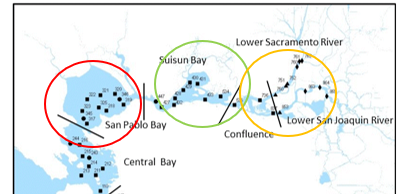
\includegraphics[width=8cm,align=m]{figures/region_map.png}
    \end{center}
  \end{Cell}
  \begin{Cell}{6}
    \vspace{0.2cm}
    \begin{center}
      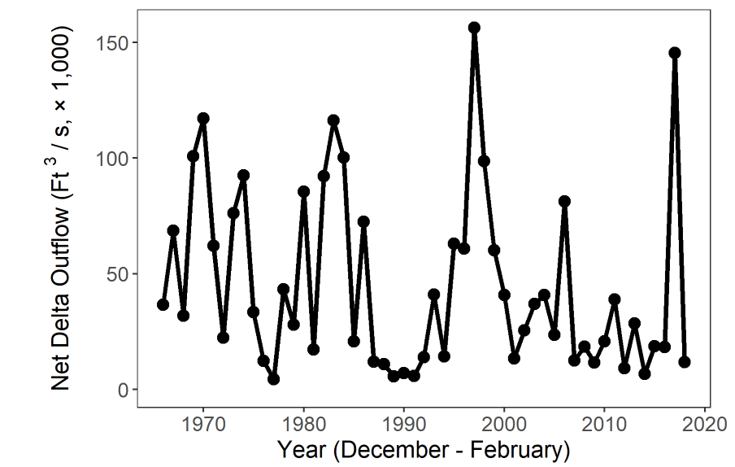
\includegraphics[width=7cm,trim=0 0 0 0,clip,align=m]{figures/outflow_tmp.png}
      \begin{itemize}[leftmargin=*]
        \item Delta outflow is a major ecosystem driver and depends on natural 
        hydrological variability and water management operations, including exports 
        from the Delta and reservoir operations. 
      \end{itemize}
    \end{center}
  \end{Cell}
\end{Row}

\vspace{1cm}

\begin{Row}
  \begin{Cell}{7}
    \begin{center}
      \begin{itemize}[leftmargin=1cm,rightmargin=1cm]
        \item Here's some info on zooplankton.
      \end{itemize}
      \vspace{0.5cm}
      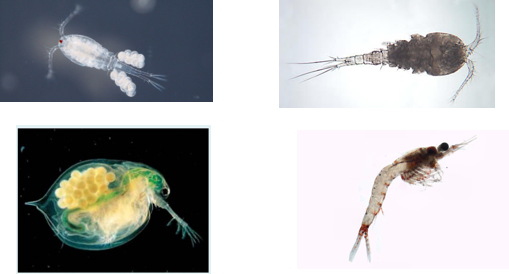
\includegraphics[width=9cm,align=m]{figures/zoop/zoop_photos.png}
    \end{center}
  \end{Cell}
  \begin{Cell}{6}
    \begin{center}
      {\bf {\large Suisun Bay}}
      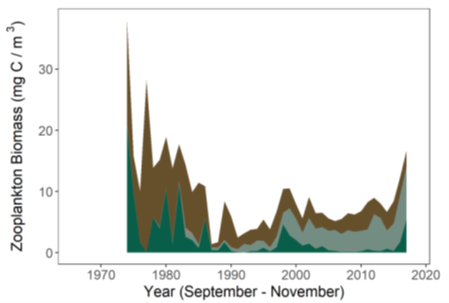
\includegraphics[width=9.5cm,align=m]{figures/zoop/zoop_suisun_bay_tmp.png}
      \vspace{0.5cm}
      \begin{itemize}[leftmargin=2cm,rightmargin=0.5cm]
        \item There used to be lots of mysids, but now it's mostly cyclopoids.
      \end{itemize}
    \end{center}
  \end{Cell}
\end{Row}

\vspace{1cm}

\begin{Row}
  \begin{Cell}{7}
    \begin{center}
      {\bf {\large The Delta}}
      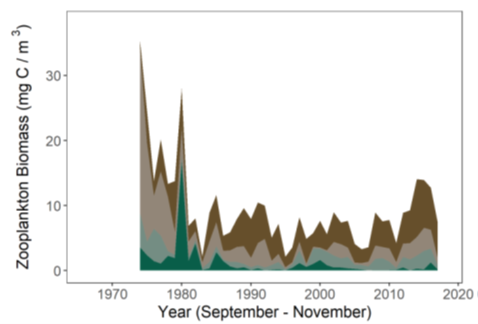
\includegraphics[width=9.5cm,align=m]{figures/zoop/zoop_delta_tmp.png}
      \vspace{0.5cm}
      \begin{itemize}[leftmargin=2cm,rightmargin=0.5cm]
        \item Lots of calanoid copepods.
      \end{itemize}
    \end{center}
  \end{Cell}
  \begin{Cell}{6}
    \begin{center}
      {\bf {\large San Pablo Bay}}
      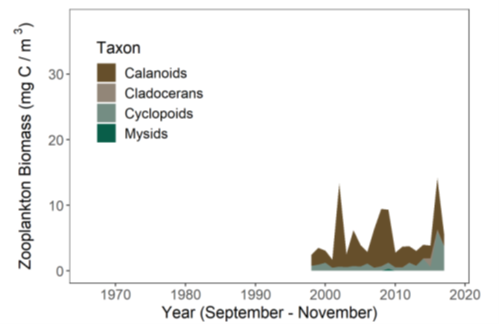
\includegraphics[width=9.5cm,align=m]{figures/zoop/zoop_san_pablo_bay_tmp.png}
      \vspace{0.5cm}
      \begin{itemize}[leftmargin=2cm,rightmargin=0.5cm]
        \item Not many zoops here.
      \end{itemize}
    \end{center}
  \end{Cell}
\end{Row}


\newpage


%%%% Smelt:
\begin{Row}
  \begin{Cell}{7}
    \vspace{0.2cm}
    \begin{center}
      \doublespacing
      {\Large Interagency Ecological Program Status \& Trends } \\
      \vspace{0.2cm}
      {\Large 2017-2018 Winter Season Report} \\
      \vspace{0.5cm}
      {\Huge Smelt} \\
      \vspace{0.3cm}
      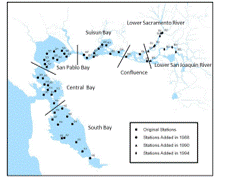
\includegraphics[width=7cm,align=m]{figures/smelt/map.png}
    \end{center}
  \end{Cell}
  \begin{Cell}{6}
    \vspace{0.2cm}
    \begin{center}
      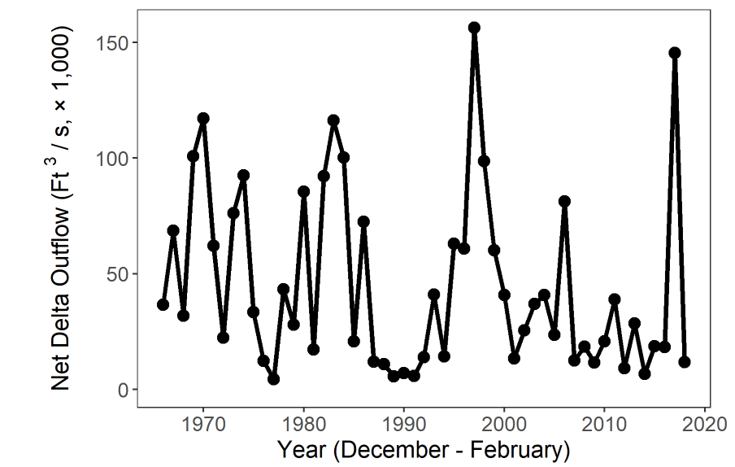
\includegraphics[width=7cm,trim=0 0 0 0,clip,align=m]{figures/outflow_tmp.png}
      \begin{itemize}[leftmargin=*]
        \item High outflow leads to increased abundance of Longfin Smelt.
        \item High outflow increases abundance of Delta Smelt only in cooler years.
      \end{itemize}
    \end{center}
  \end{Cell}
\end{Row}

\vspace{0.5cm}

\begin{Row}
  \begin{Cell}{7}
    \begin{center}
      {\bf {\large Longfin Smelt – Bay Study}}
    \end{center}
  \end{Cell}
  \begin{Cell}{6}
    \begin{center}  
      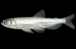
\includegraphics[align=m]{figures/smelt/photo_longfin_smelt.png}
    \end{center}
  \end{Cell}
\end{Row}

\begin{Row}
  \begin{Cell}{7}
    \begin{center}
      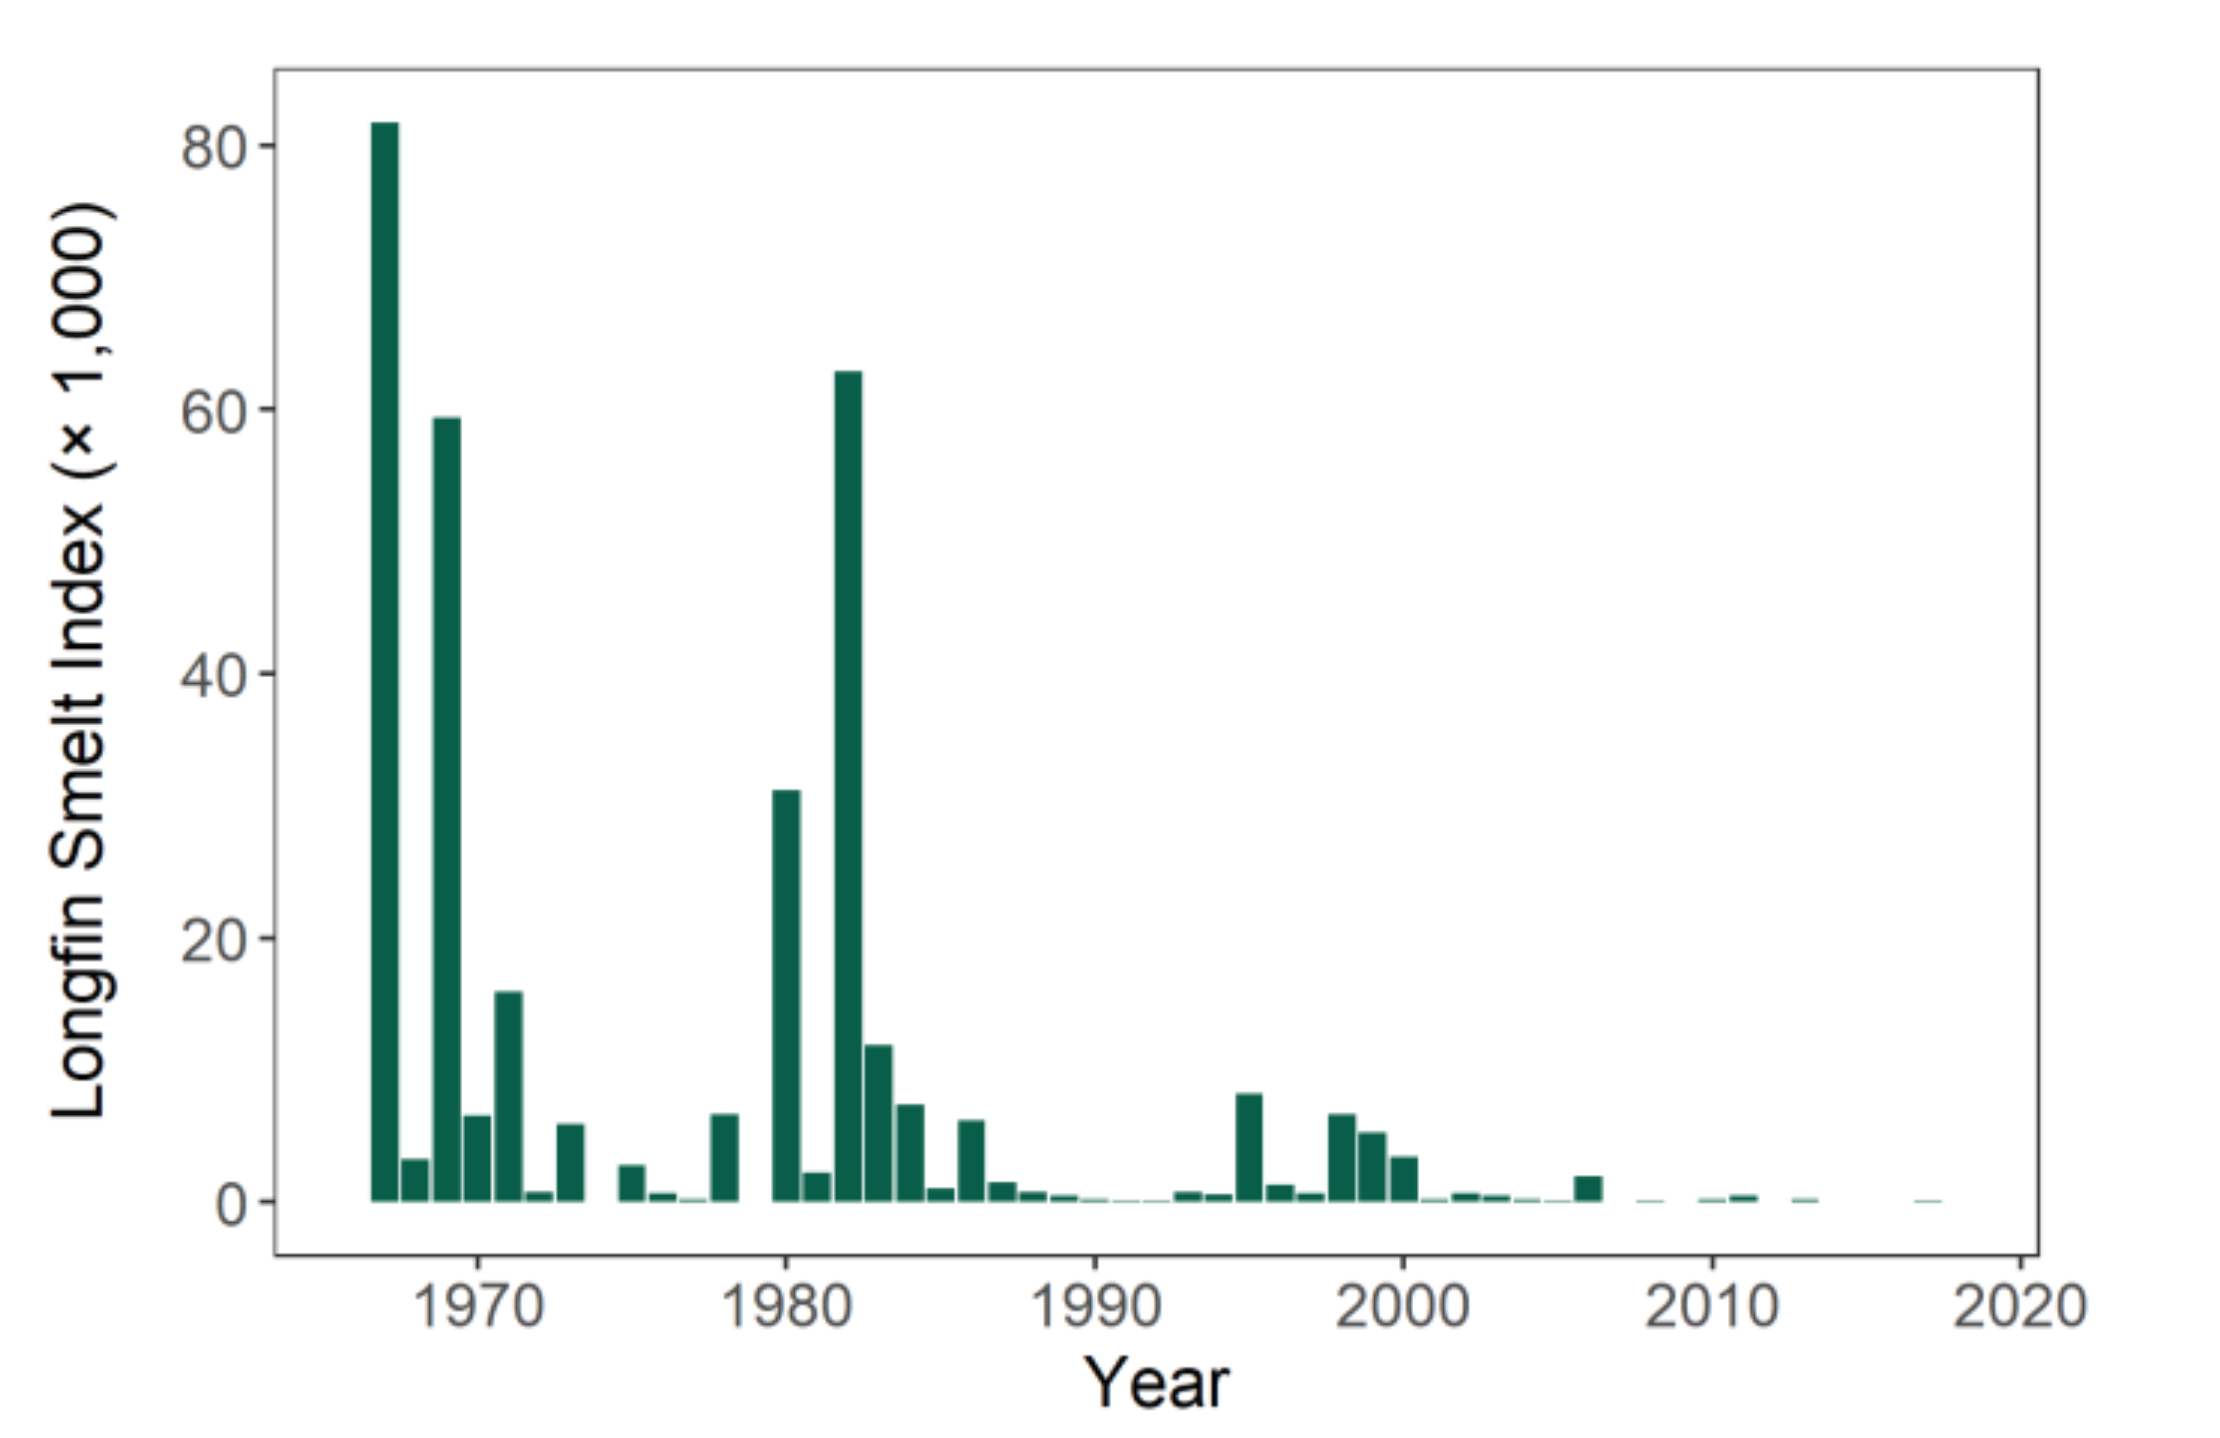
\includegraphics[width=10cm,trim=0 0 0 40,clip,align=m]{figures/smelt/longfin_tmp.png}
    \end{center}
  \end{Cell}
  \begin{Cell}{6}
    \begin{center}
      \vspace{-3cm}
      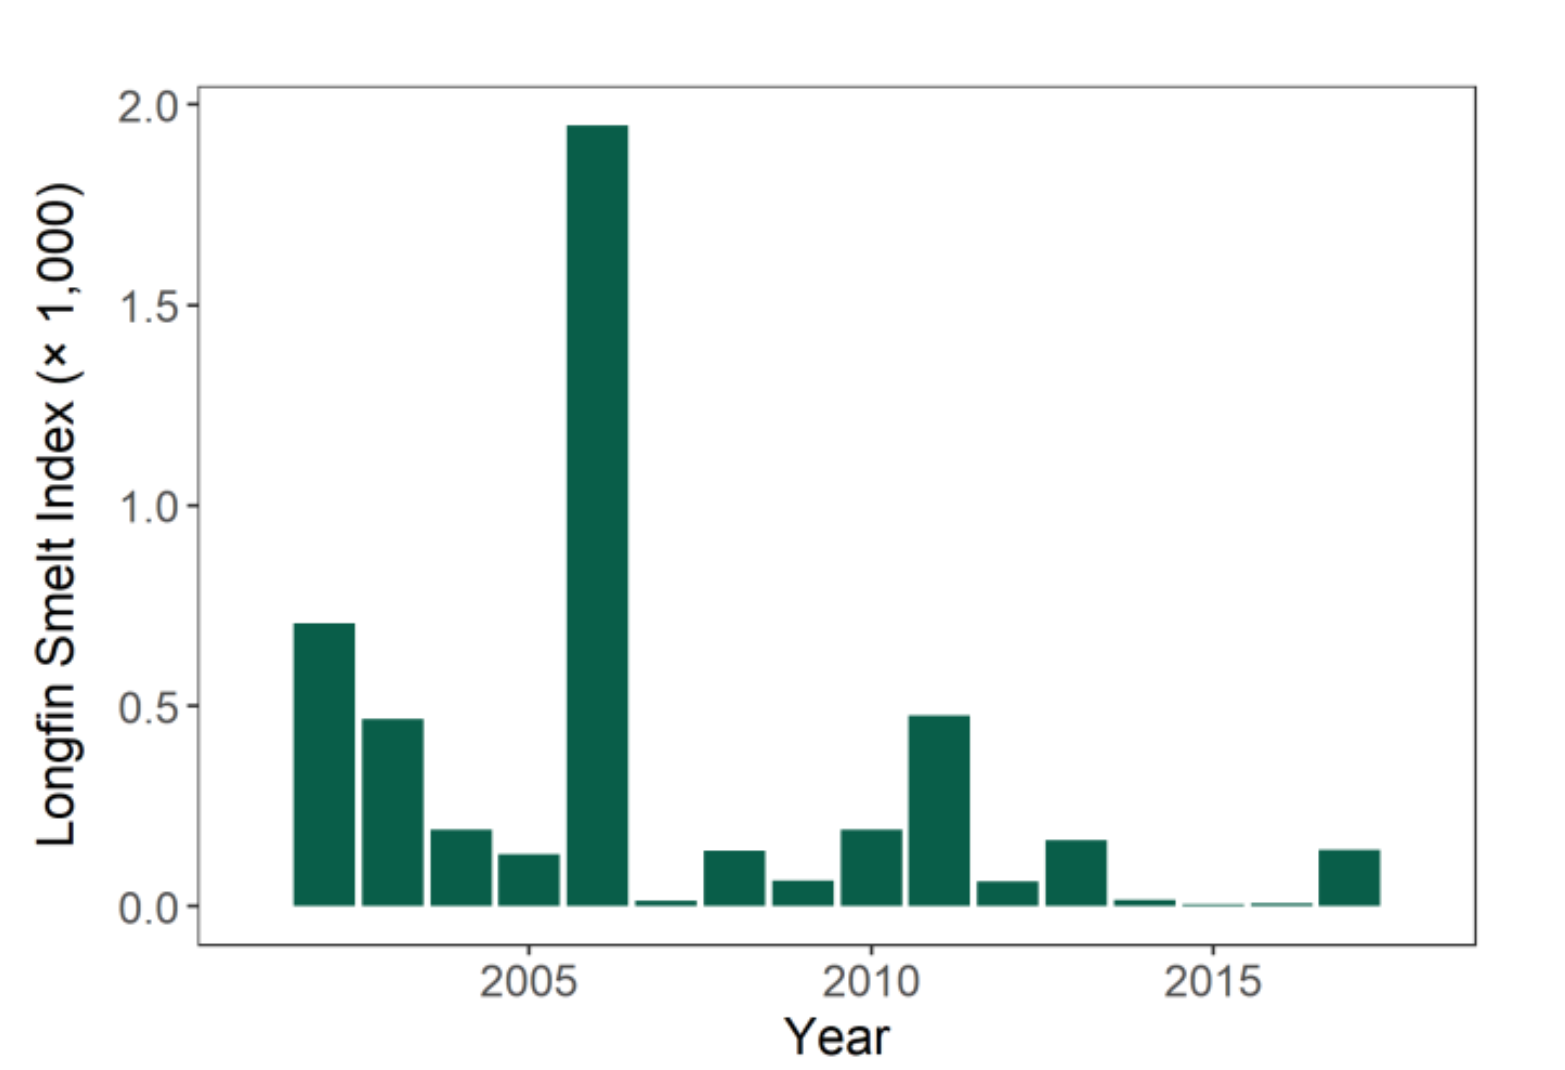
\includegraphics[width=7cm,trim=0 0 0 50,clip,align=m]{figures/smelt/longfin_tmp_2.png}
      \begin{itemize}[leftmargin=*]
        \item Longfin smelt experienced sever declines in the early 2000s and have 
        not recovered. 
        \item Bay Study is the only IEP survey that samples throughout San Francisco Bay, 
        making it especially good at pickup up Longfin Smelt.
      \end{itemize}
    \end{center}
  \end{Cell}
\end{Row}

\vspace{0.5cm}

\begin{Row}
  \begin{Cell}{7}
    \begin{center}
      {\bf {\large Delta Smelt – SKT}}
    \end{center}
  \end{Cell}
  \begin{Cell}{6}
    \begin{center}
      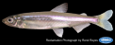
\includegraphics[align=m]{figures/smelt/photo_delta_smelt.png}
    \end{center}
  \end{Cell}
\end{Row}

\begin{Row}
  \begin{Cell}{7}
    \begin{center}
      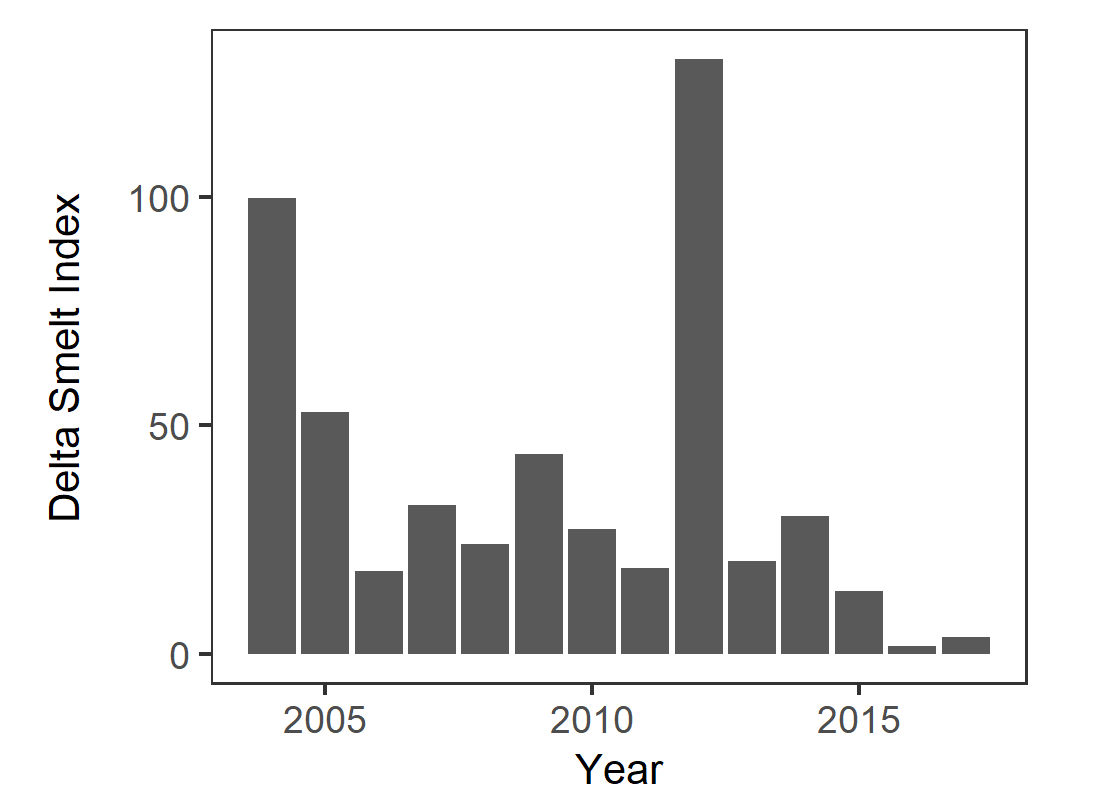
\includegraphics[width=10cm,align=m]{figures/smelt/skt_dsm_fig.png}
    \end{center}
  \end{Cell}
  \begin{Cell}{6}
    \begin{center}
      \vspace{-3cm}
      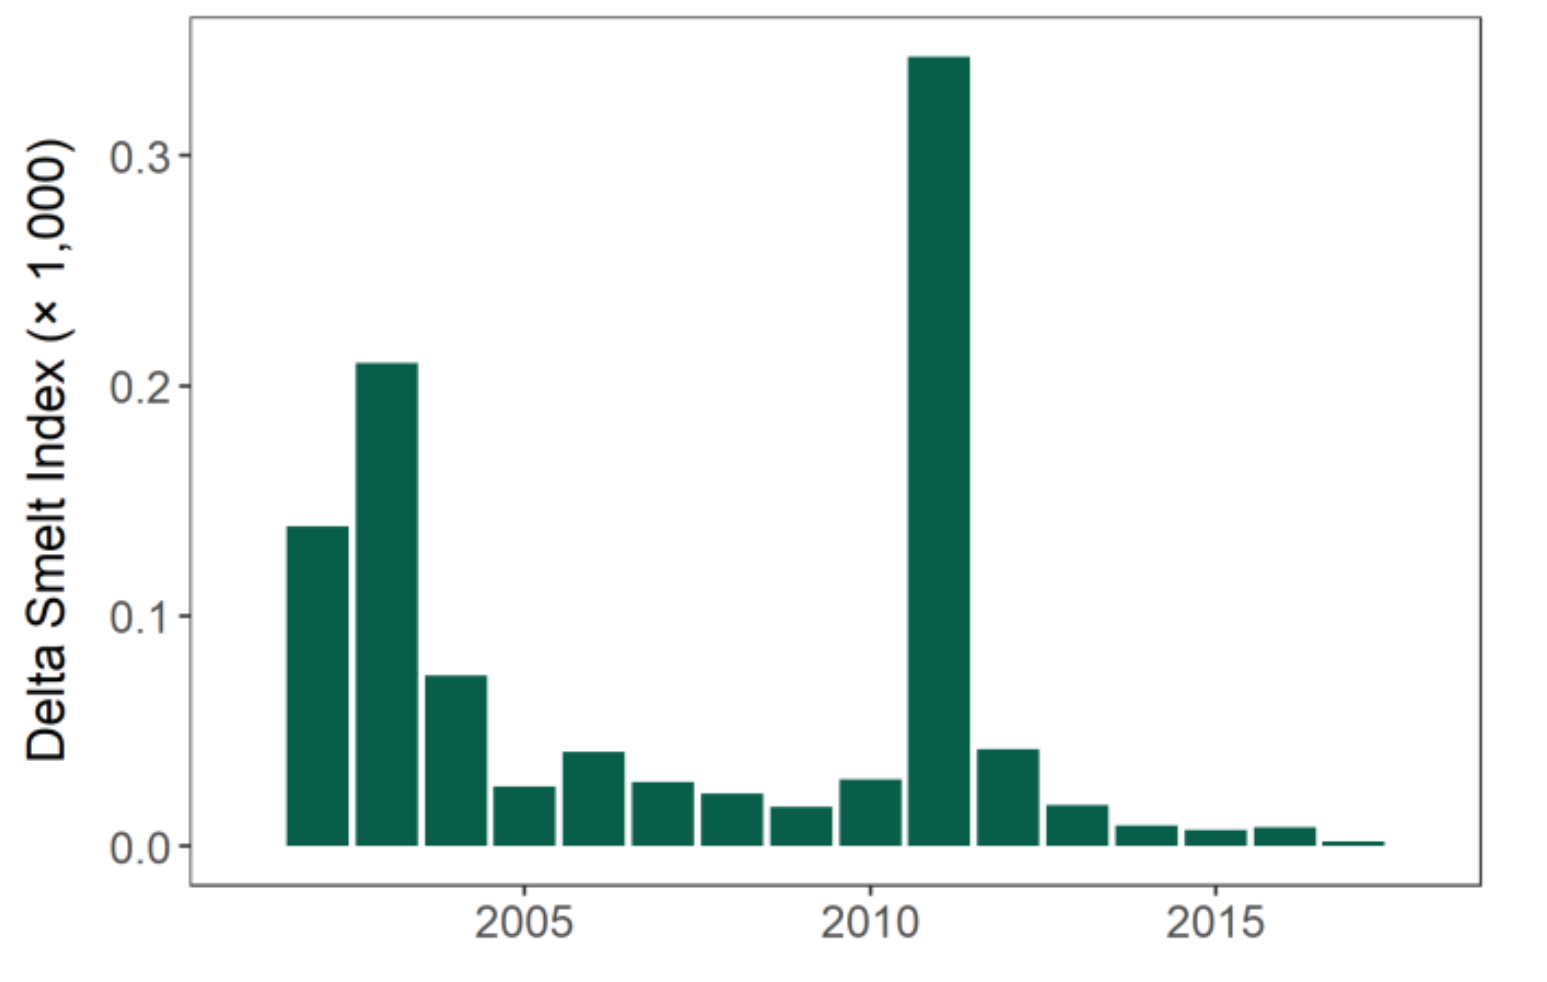
\includegraphics[width=7cm,align=m]{figures/smelt/delta_smelt_tmp_2.png}
      \begin{itemize}[leftmargin=*]
        \item Spring Kodiak Trawl samples throughout the Bay and Delta.
        \item Delta smelt are not doing so great.
      \end{itemize}
    \end{center}
  \end{Cell}
\end{Row}


\newpage


%%%% Salmon:
\begin{Row}
  \begin{Cell}{7}
    \vspace{0.2cm}
    \begin{center}
      \doublespacing
      {\Large Interagency Ecological Program Status \& Trends } \\
      \vspace{0.2cm}
      {\Large 2017-2018 Winter Season Report} \\
      \vspace{0.5cm}
      {\Huge Salmon} \\
      \vspace{0.3cm}
      \singlespacing
      
			\begin{minipage}{240pt}
        \begin{center}
          \begin{itemize}[leftmargin=*]
              \item Salmon have been doing OK in recent years, though not amazing.
              \item The drought was hard on them.
          \end{itemize}
        \end{center}
			\end{minipage}
      
      \vspace{1cm}
      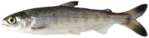
\includegraphics[width=4cm,trim=0 0 0 0,clip,align=m]{figures/salmon/photo_salmon.png}
    \end{center}
  \end{Cell}
  \begin{Cell}{6}
    \vspace{0.2cm}
    \begin{center}
      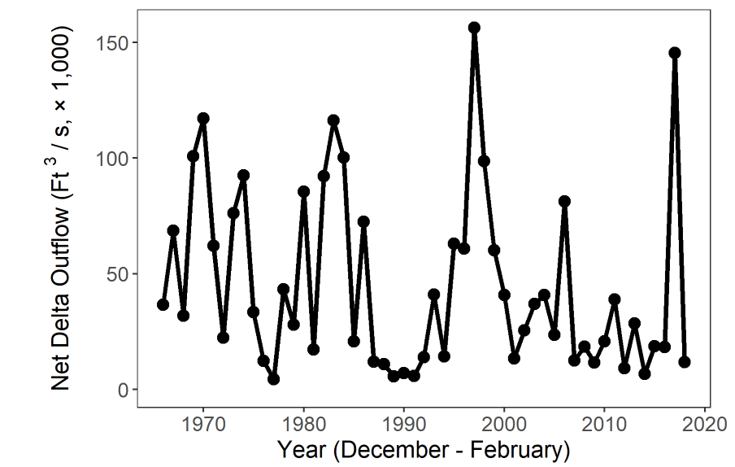
\includegraphics[width=7cm,trim=0 0 0 0,clip,align=m]{figures/outflow_tmp.png}
    \end{center}
  \end{Cell}
\end{Row}

\vspace{1cm}

\begin{Row}
  \begin{Cell}{7}
    \begin{center}
      {\bf {\large Red Bluff Diversion Dam}}
    \end{center}
  \end{Cell}
  \begin{Cell}{6}
  \end{Cell}
\end{Row}

\begin{Row}
  \begin{Cell}{7}
    \begin{center}
      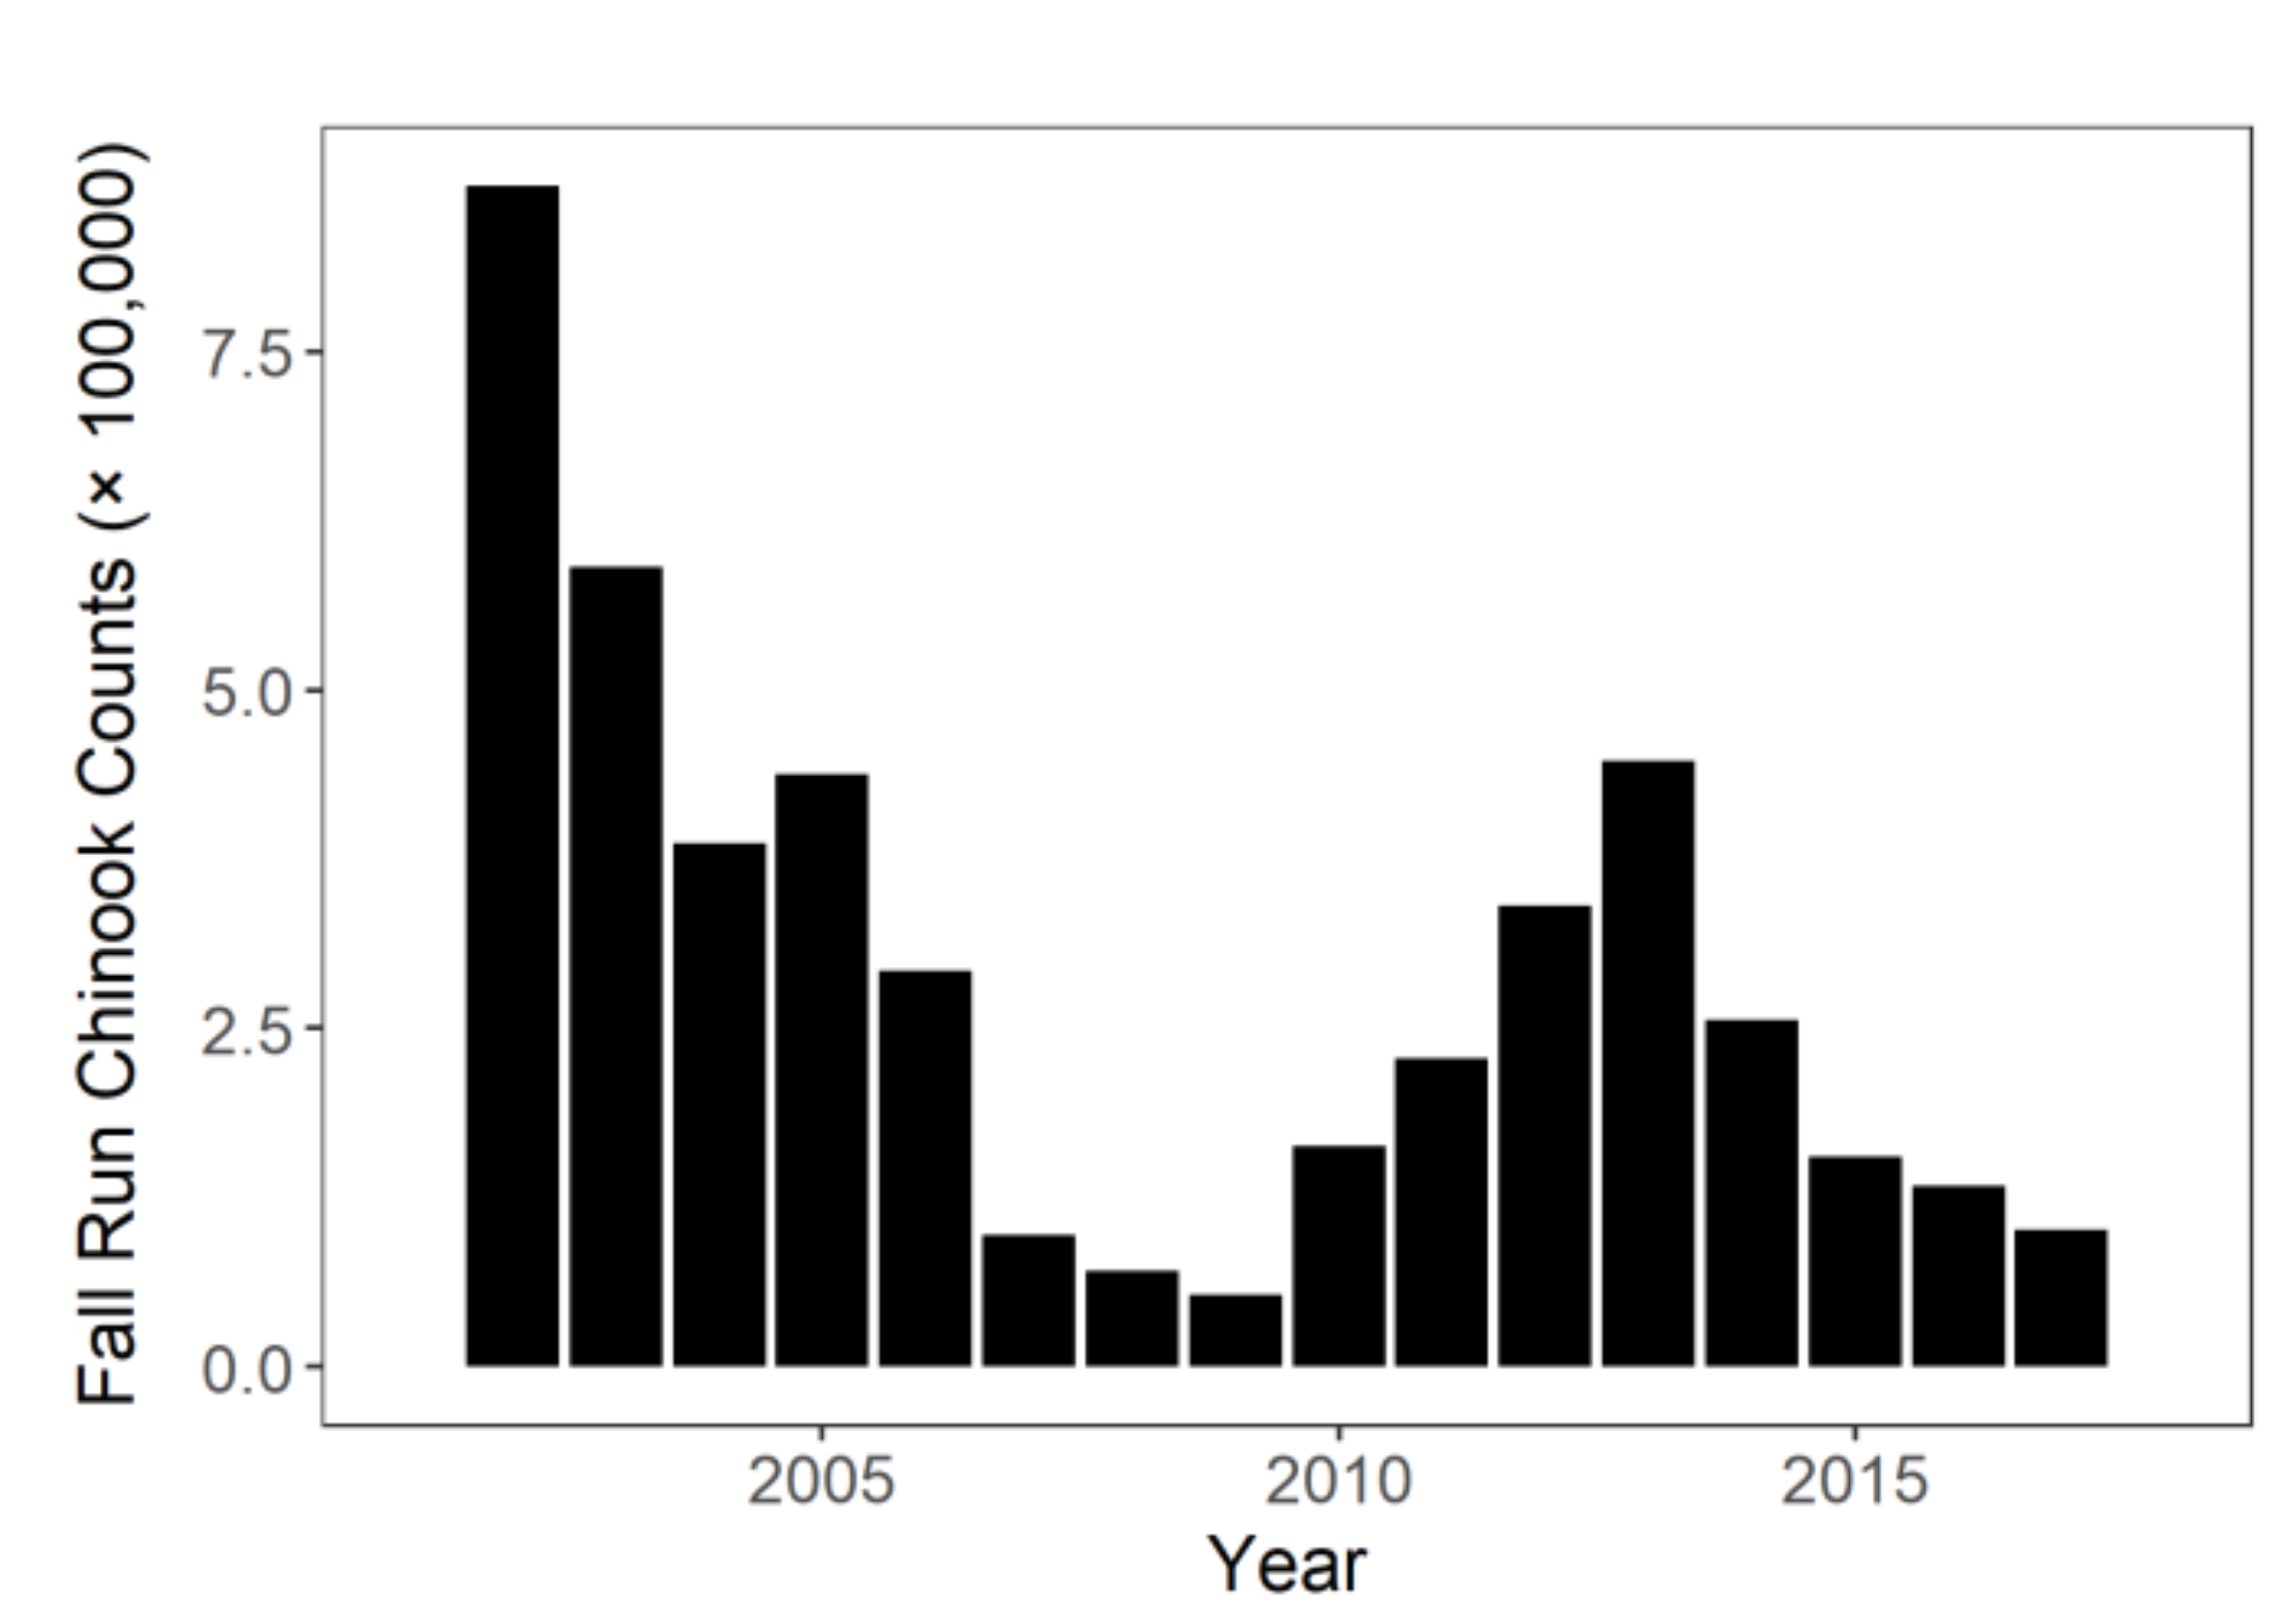
\includegraphics[width=11cm,trim=0 0 0 40,clip,align=m]{figures/salmon/red_bluff_tmp.png}
    \end{center}
  \end{Cell}
  \begin{Cell}{6}
    \vspace{-2cm}
    \begin{center}
      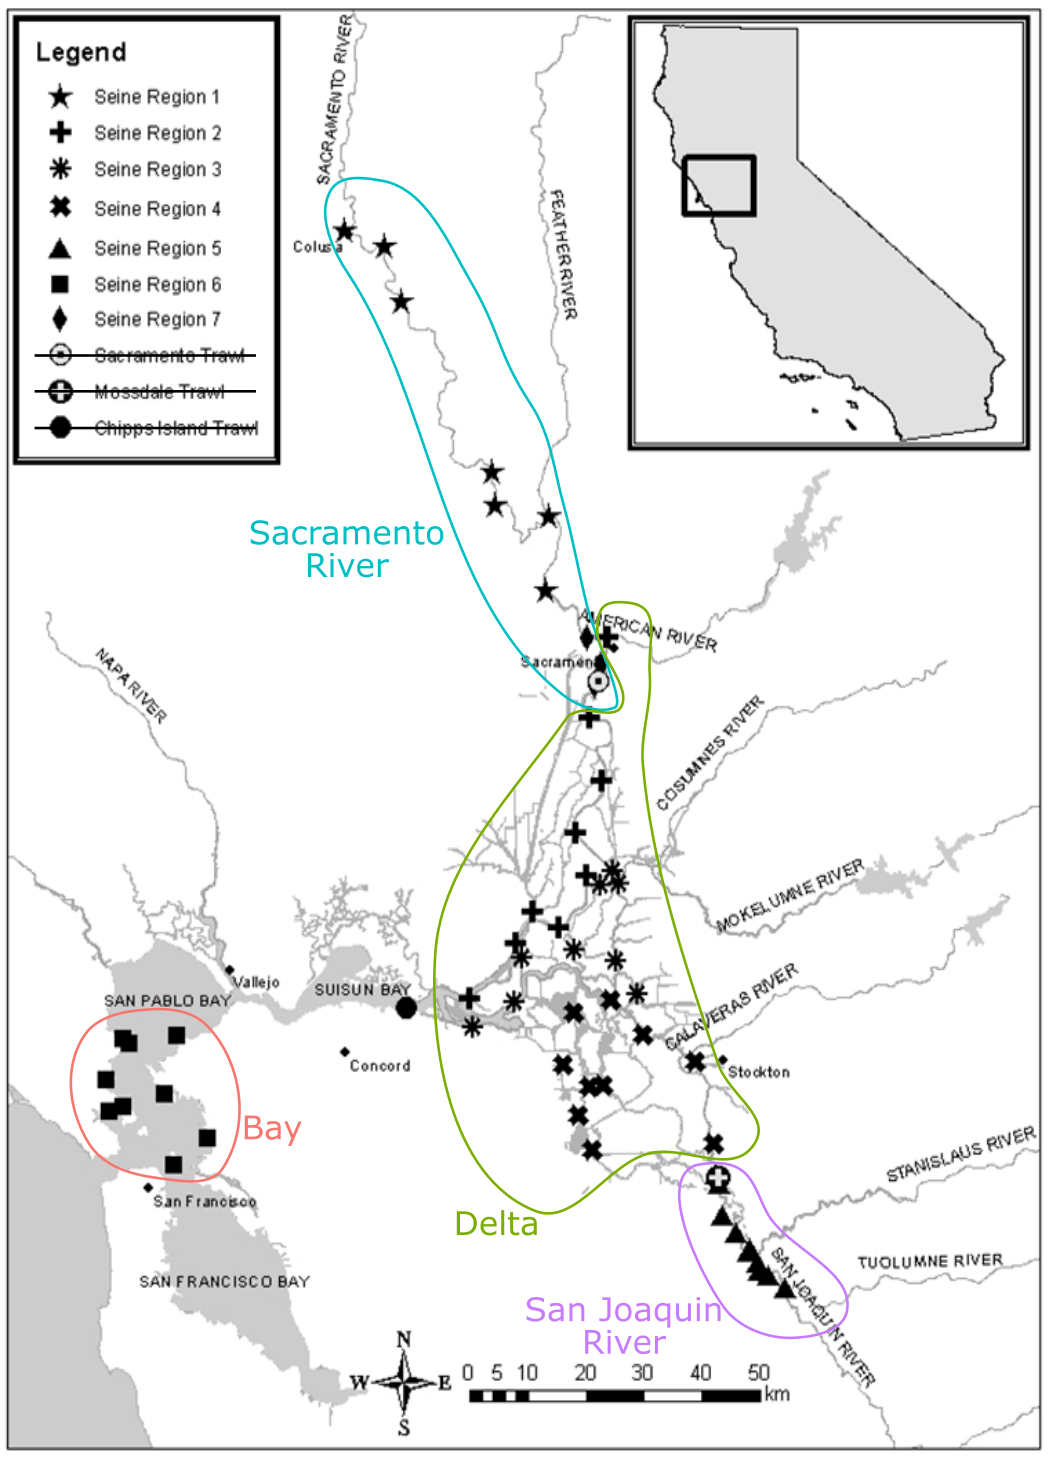
\includegraphics[width=7cm,align=m]{figures/salmon/djfmp_map_tmp_2.png}
    \end{center}
  \end{Cell}
\end{Row}

\vspace{0.5cm}

\begin{Row}
  \begin{Cell}{7}
    \begin{center}
      {\bf {\large DJFMP Beach Seines}}
    \end{center}
  \end{Cell}
  \begin{Cell}{6}
  \end{Cell}
\end{Row}

%\vspace{1cm}

\begin{Row}
  \begin{Cell}{7}
    \begin{center}
      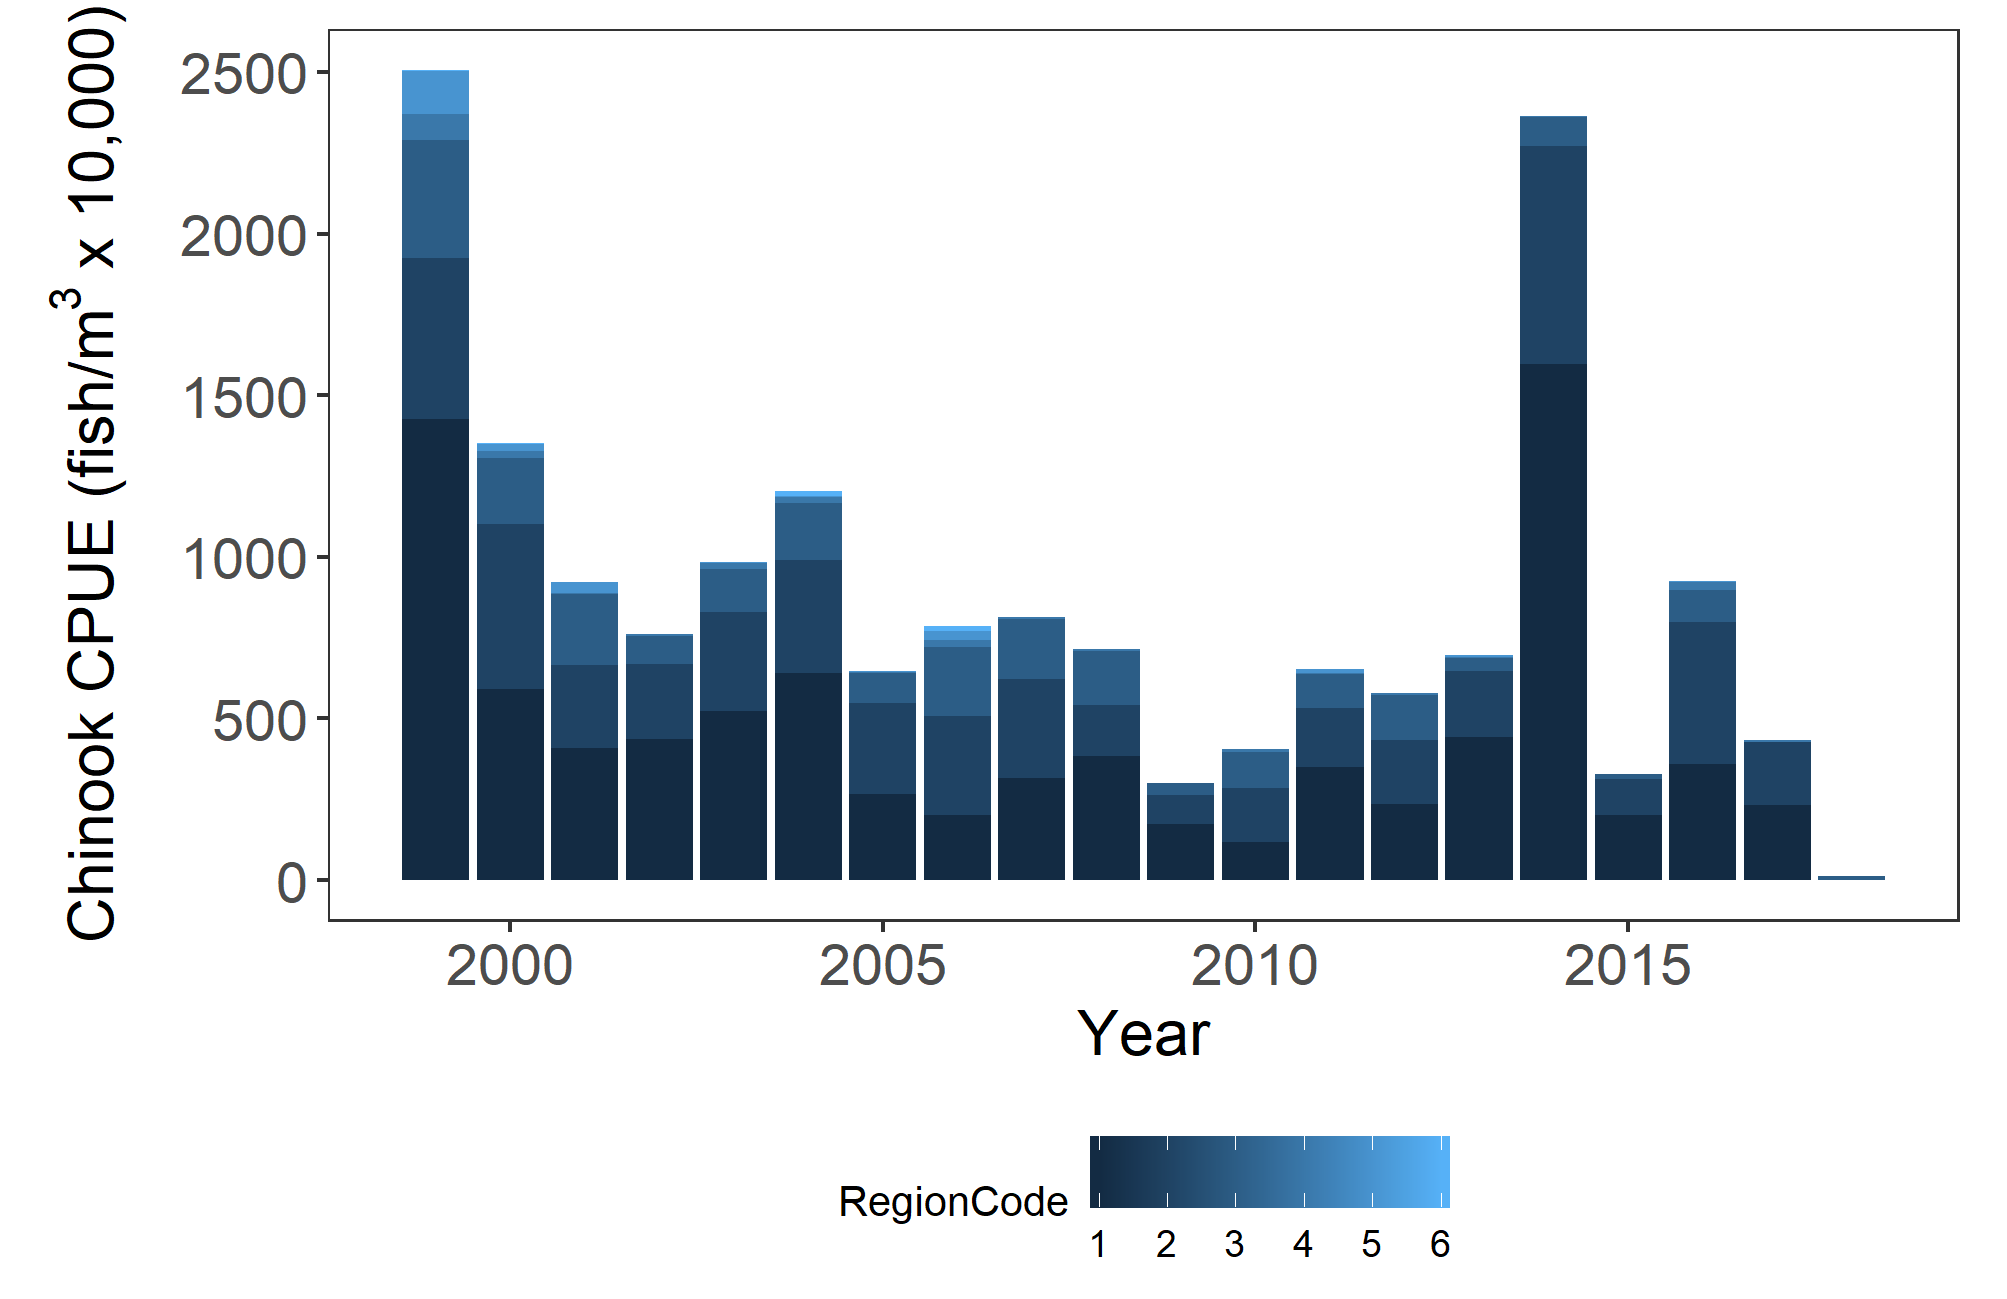
\includegraphics[width=11cm,align=m]{figures/salmon/djfmp_chn_fig.png}
    \end{center}
  \end{Cell}
  \begin{Cell}{6}
    %\vspace{-3cm}
    \begin{center}
      \begin{itemize}[leftmargin=*]
        \item Preliminary estimates of passage by brood-year (BY) and run for 
        unmarked juvenile Chinook salmon and steelhead trout captured by rotary-screw 
        traps at Red Bluff Diversion Dam (RK391), Sacramento River, CA.
        \item This sampling provides an estimate of production in the upper watershed.
      \end{itemize}
    \end{center}
    \vspace{3cm} 
    \begin{center}
      \begin{itemize}[leftmargin=*]
        \item DJFMP’s beach seine data provides information on landscape patterns of 
        juvenile chinook occurrence.
        \item Researchers use these patterns to determine differences in salmon 
        life-history.
      \end{itemize}
    \end{center}
  \end{Cell}
\end{Row}


\newpage


%%%% Other fish:
\begin{Row}
  \begin{Cell}{7}
    \vspace{0.2cm}
    \begin{center}
      \doublespacing
      {\Large Interagency Ecological Program Status \& Trends } \\
      \vspace{0.2cm}
      {\Large 2017-2018 Winter Season Report} \\
      \vspace{0.5cm}
      {\Huge Other fish} \\
      \vspace{0.3cm}
      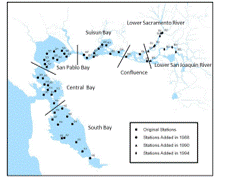
\includegraphics[width=7cm,align=m]{figures/smelt/map.png}
    \end{center}
  \end{Cell}
  \begin{Cell}{6}
    \vspace{0.2cm}
    \begin{center}
      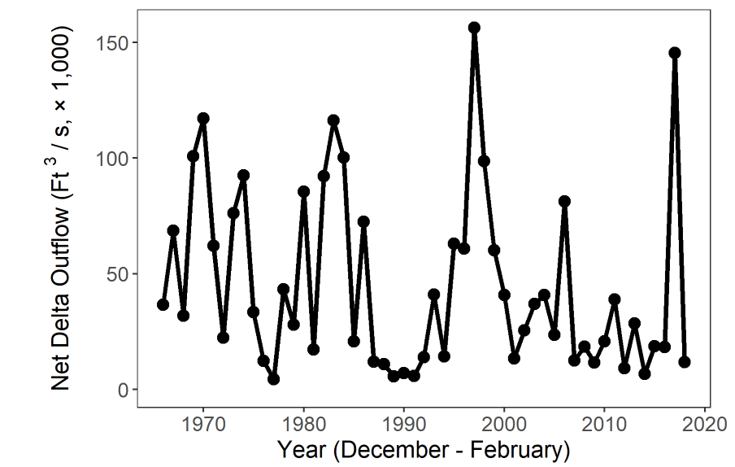
\includegraphics[width=7cm,trim=0 0 0 0,clip,align=m]{figures/outflow_tmp.png}
      %\begin{itemize}[leftmargin=*]
      %\end{itemize}
    \end{center}
  \end{Cell}
\end{Row}

\vspace{0.5cm}

\begin{Row}
  \begin{Cell}{7}
    \begin{center}
      {\bf {\large Splittail – Yolo bypass screw trap}}
      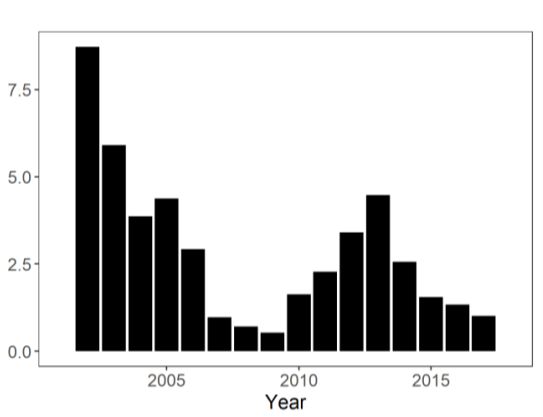
\includegraphics[align=m]{figures/otherfish/splittail_yb_tmp.png}
    \end{center}
  \end{Cell}
  \begin{Cell}{6}
    \begin{center}
      \vspace{1cm}
      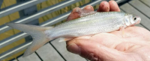
\includegraphics[width=7cm,align=m]{figures/otherfish/splittail_photo.png}
      \vspace{1.5cm}
      \begin{itemize}[leftmargin=*]
        \item Splittail spawn on flood plains such as the yolo bypass.
        \item They do really well in wet years. 
        \item The screw trap catches a lot of juvenile splittail in the spring after 
        a wet year.
      \end{itemize}
    \end{center}
  \end{Cell}
\end{Row}

\vspace{0.5cm}

\begin{Row}
  \begin{Cell}{7}
    \begin{center}
      \vspace{-2cm}
      {\bf {\large Sturgeon – Bay Study}}
      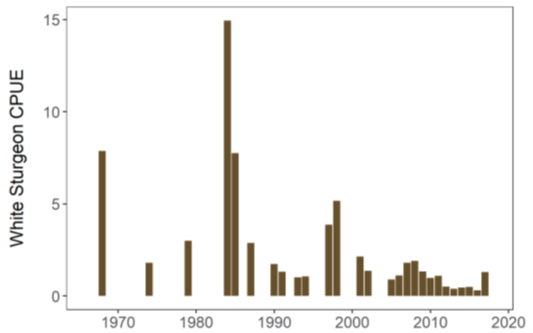
\includegraphics[align=m]{figures/otherfish/sturgeon_bay_study.png}
    \end{center}
  \end{Cell}
  \begin{Cell}{6}
    \begin{center}
      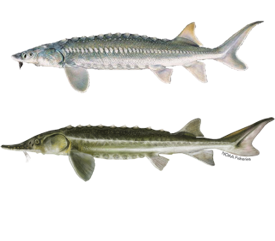
\includegraphics[width=7cm,align=m]{figures/otherfish/sturgeon_figs.png}
      \vspace{-0.5cm}
      \begin{itemize}[leftmargin=*]
        \item Juvenile sturgeon are caught in Bay Study’s otter trawl.
        \item White sturgeon support a recreational fishery.
        \item Green sturgeon are listed as threatened.
      \end{itemize}
    \end{center}
  \end{Cell}
\end{Row}



%\begin{Row}
%  \begin{Cell}{2}
%    \setlength{\fboxrule}{1.7pt}
%    \fcolorbox{black}[HTML]{FFEEBA}{\parbox{\textwidth}{
%			\begin{itemize}[leftmargin=*]
%				{\large 
%					\item IEP has collected water quality data since 1975 as mandated by state 
%					and federal regulations. 
%					\item Delta outflow (at right) is a major ecosystem driver and depends on 
%					natural hydrological variability and water management operations, including 
%					exports from the Delta and reservoir operations.
%					\item Organisms in this ecosystem are adapted to high turbidity conditions, 
%					and reductions in turbidity can have many negative ecological effects. 
%					Higher values for Secchi depth indicate lower turbidity.
%					\item Dissolved inorganic nitrogen (DIN) affects primary productivity, with 
%					different forms having different effects. DIN, particularly ammonium, is 
%					predicted to decline significantly over the next five years in response to 
%					wastewater treatment plant system upgrades.
%				}
%			\end{itemize}
%    }}
%  \end{Cell}
%  \begin{Cell}{1}
%    \vspace{-4.0cm}
%    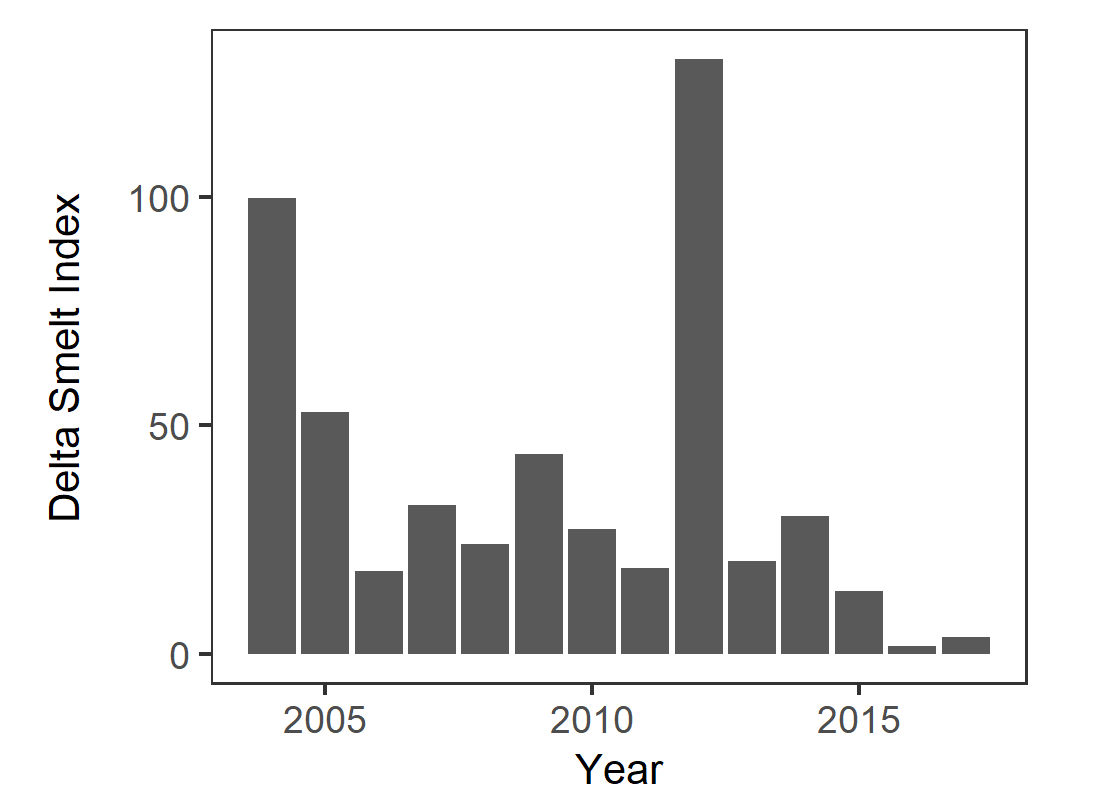
\includegraphics[align=m]{figures/smelt/skt_dsm_fig.PNG}
%		%<<skt_dsm_fig, results="asis", echo=FALSE, fig.height=4, fig.width=6, message=FALSE, warning=FALSE>>=	
%		%	plot(skt_dsm_fig)
%		%@
%  \end{Cell}
%\end{Row}

%\vspace{-0cm}

%\begin{Row}
%   \begin{Cell}{1}
%			\hspace{42pt}
%			\begin{minipage}{195pt}
%				\fcolorbox{black}[HTML]{27408B}{\parbox[c][12pt]{\textwidth}{
%					\begin{center}
%						{\LARGE \textcolor{white}{San Pablo Bay}}
%					\end{center}
%				}}
%			\end{minipage}% This must go next to `\end{minipage}`
%			\hspace{62pt}
%			\begin{minipage}{195pt}
%				\fcolorbox{black}[HTML]{27408B}{\parbox[c][12pt]{\textwidth}{
%					\begin{center}
%						{\LARGE \textcolor{white}{Suisun Bay}}
%					\end{center}
%				}}
%			\end{minipage}% This must go next to `\end{minipage}`			
%			\hspace{62pt}
%			\begin{minipage}{195pt}
%				\fcolorbox{black}[HTML]{27408B}{\parbox[c][12pt]{\textwidth}{
%					\begin{center}
%						{\LARGE \textcolor{white}{Delta}}
%					\end{center}
%				}}
%			\end{minipage}
%   \end{Cell}
%\end{Row}

%\vspace{-0.2cm}

%\begin{Row}
%    \begin{Cell}{1}
%      %\includegraphics[align=m,width=1.0\textwidth]{figures/main_fig.PNG}
%			%<<water_quality_main_fig, results="asis", echo=FALSE, fig.height=5.3, fig.width=12>>=
%			%	plot(water_quality_main_fig)
%			%@
%		\end{Cell}
%\end{Row}

%\vspace{0.2cm}

%\begin{Row}
%    \begin{Cell}{14}
%      \textbf{\underline{FOR MORE INFORMATION}}: The 
%			\href{https://water.ca.gov/Programs/Environmental-Services/Compliance-Monitoring-And-Assessment/Dayflow-Data}{California Estuary Portal} 
%			provides access to raw and summarized water quality data for the 
%			Sacramento-San Joaquin Delta. The 
%			\href{https://water.ca.gov/Programs/Environmental-Services/Compliance-Monitoring-And-Assessment/Dayflow-Data}{California Department of Water Resources} 
%			provides information and data on outflow. The IEP website provides the 
%			\href{https://water.ca.gov/-/media/DWR-Website/Web-Pages/Programs/Environmental-Services/Interagency-Ecological-Program/Files/Interagency-Ecological-Program-Status-and-Trends-Fall-2017.pdf}{metadata} 
%			for production of this report.
%    \end{Cell}
%    \begin{Cell}{2}
%
%    \end{Cell}
%\end{Row}



\end{document}
